\chapter{CellTAN Application}

\section{MPPT Curve}

\begin{figure}[h]
    \centering
    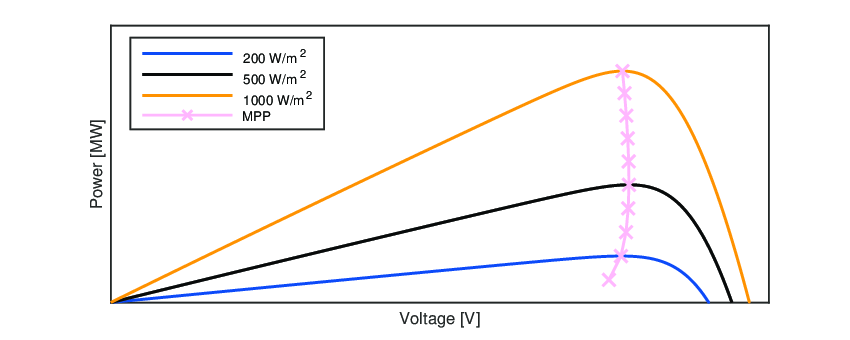
\includegraphics[width=14cm]{figures/appendix/b_analysis/mpptcurve.png} \caption{"PV panel power characteristics as a function of the DC voltage and solar irradiance."} Image source and copyright: \cite{lunardi}.
    \label{fig:mpptcurve}
\end{figure}

\section{Data analysis} \label{ap2:eda}


\begin{figure}[h]
    \centering
    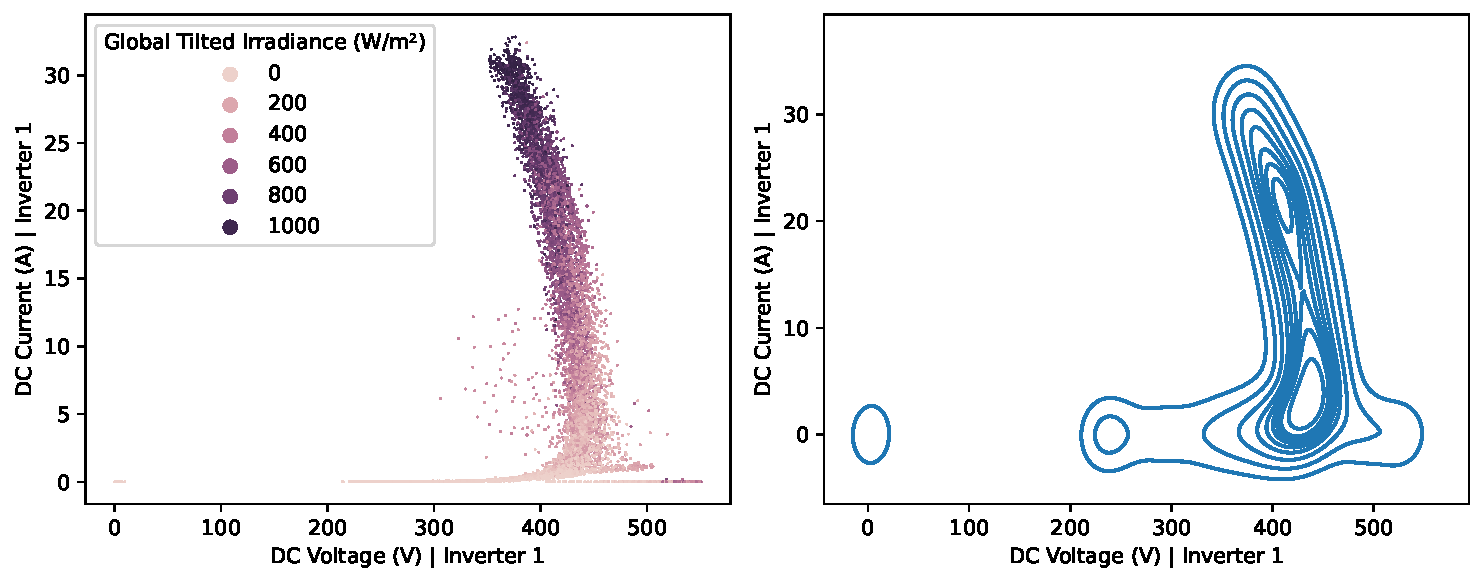
\includegraphics[width=\textwidth]{figures/appendix/b_analysis/05_voltage_current_pairplot_test_1.pdf}
    \caption{Pair plot of DC side voltage and current from inverter one (2023), using scatter (left) and KDE (Kernel Density Estimation) (right).}
    \label{fig:eda_voltage_current_test_1}
\end{figure}

\begin{figure}[h]
    \centering
    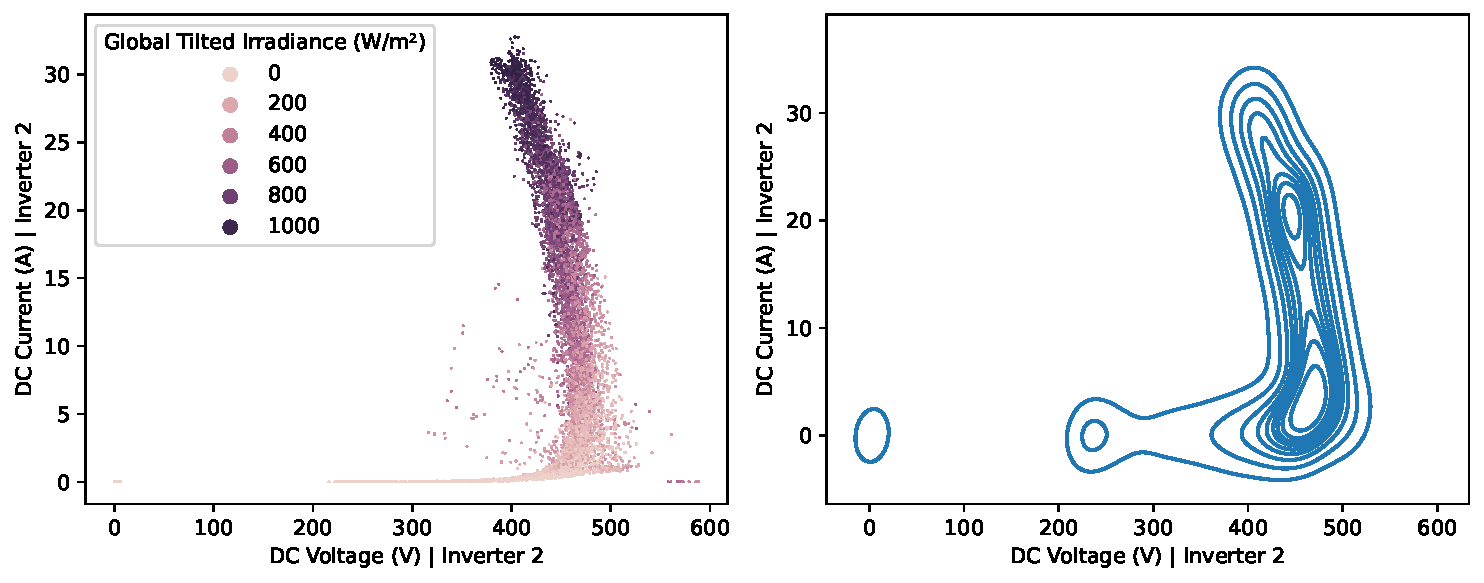
\includegraphics[width=\textwidth]{figures/appendix/b_analysis/07_voltage_current_pairplot_test_2.pdf}
    \caption{Pair plot of DC side voltage and current from inverter two (2023), using scatter (left) and KDE (Kernel Density Estimation) (right).}
    \label{fig:eda_voltage_current_test_2}
\end{figure}

\begin{figure}[h]
    \centering
    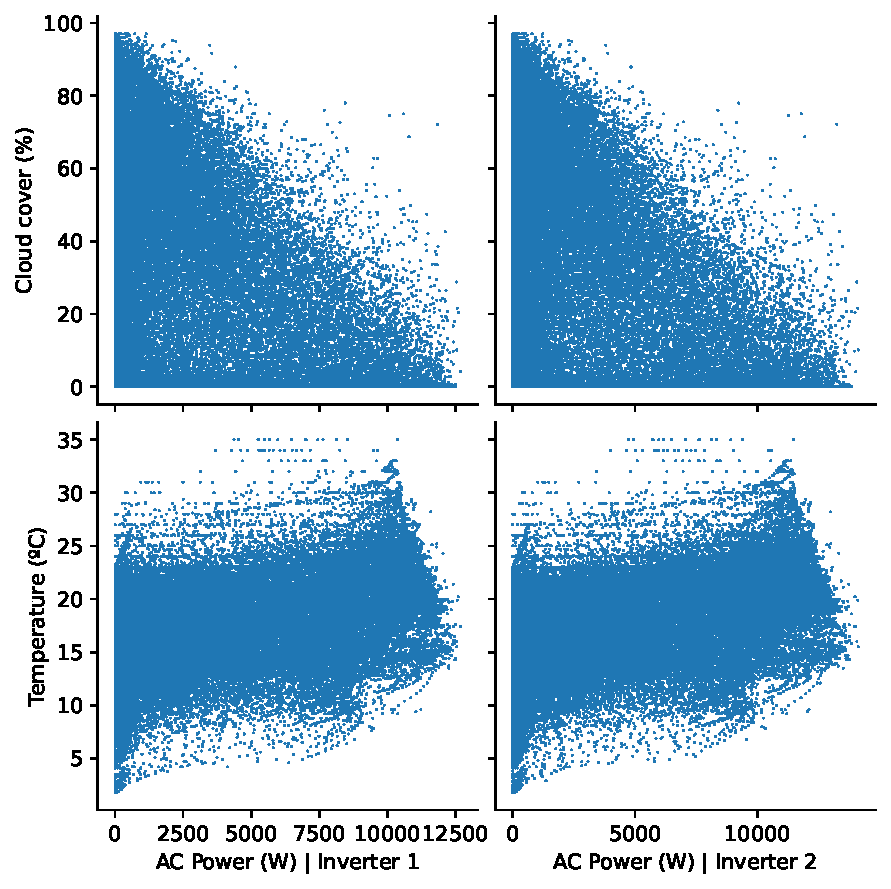
\includegraphics[width=0.6\textwidth]{figures/appendix/b_analysis/12_power_meteo_pairplot_kb.pdf}
    \caption{Scatter pair-plot of AC power from the two inverters with cloud coverage and temperature (from satellite).}
    \label{fig:eda_irrelevant_meteo}
\end{figure}

